\section{Heap Sort} \label{cap:2:section:hsort}

\subsection{Introdução}

O \textit{Heap} Sort é um algoritmo de ordenação bastante eficiente, seu funcionamento é baseado
na estrutura de dados chamada \textit{Heap}, que pode ser implementada utilizando um vetor que
mantém as propriedades de \textit{Heap}, seja ela a propriedade de \textit{max-heap} ou a propriedade
de \textit{min-heap}.

\begin{itemize}

    \item \textit{max-heap}: é uma propriedade da estrutura de dados \textit{Heap} que indica que
    a raiz ou primeiro indíce do vetor é o maior elemento da \textit{Heap}.
    \item \textit{min-heap}: é uma propriedade da estrutura de dados \textit{Heap} que indica que
    a raiz ou primeiro indíce do vetor é o menor elemento da \textit{Heap}.

\end{itemize}

\subsection{Implementação}

Para o algoritmo de ordenação baseado na estrutura de uma \textit{Heap}, o pseudo-código utilizado para desenvolver o
algoritmo pode ser observado em \ref{heapSortP}.

\begin{pseudocode}[caption={Algoritmo de ordenação utilizando uma \textit{Heap}}, label={heapSortP}]
HEAP-SORT(A)
n $\gets$ len(A)
BUILD-MAX-HEAP(A)
i $\gets$ n - 1
while i > 1 do
    swap(A[0], A[i])
    MAX-HEAPIFY(A)
    i $\gets$ i - 1
\end{pseudocode}

Esse pseudo-código foi implementado na linguagem de programação C 
e pode ser observado no código seguinte:

\begin{lstlisting}[style=CStyle]
void heapify(int * v, int n, int i)
{

    int largest = i;

    int left = 2 * i + 1;

    int right = 2 * i + 2;

    if (left < n && v[left] > v[largest])
    {
        largest = left;
    }

    if (right < n && v[right] > v[largest])
    {
        largest = right;
    }

    if (largest != i)
    {
        swap(&v[i], &v[largest]);

        heapify(v, n, largest);
    }
}

void hSort(int * v, int n)
{
    int i;

    for (i = n / 2 - 1; i >= 0; i--)
    {
        heapify(v, n, i);
    }

    // Heap sort
    for (int i = n - 1; i > 0; i--) 
    {

        swap(&v[0], &v[i]);

        heapify(v, i, 0);
    }
}
\end{lstlisting}

\subsection{Análise do algoritmo e notação assintótica}

Para que seja determinada a razão de crescimento do algoritmo de ordenação pela estrutura da \textit{Heap}, é necessário
perceber os tempos de execução de cada linha do pseudo-código \ref{heapSortP}.
Nesse caso, pode-se ter como base a equação \ref{cap:2:eq:heapSort:1}.

\begin{equation} \label{cap:2:eq:heapSort:1}
    T(n) = C_2 + T(BUILDMAXHEAP) + C_4 + \sum_{i=2}^{n - 1}(C_6 + T(MAXHEAPIFY) + C_8)
\end{equation}

Sabendo que, o tempo de execução $T(BUILDMAXHEAP) = O(n)$ e o tempo de execução $T(MAXHEAPIFY) = O(\log n)$, podemos assumir
a relação entre a equação \ref{cap:2:eq:heapSort:1} com a equação \ref{cap:2:eq:heapSort:2}.

\begin{equation} \label{cap:2:eq:heapSort:2}
    T(n) = n + an + c\  para\  a = (C_6 + \log n + C_8)\  e\  c = (C_2 + C_4)
\end{equation}

Com isso, pode-se determinar as seguintes notações assintóticas para o algoritmo de ordenação 
pela estrutura da \textit{Heap}:

\begin{align*} \label{cap:2:eq:heapSort:3}
    O(n) &= n \times \log n \\ 
    \Omega(n) &= n \times \log n \\
    \Theta(n) &= n \times \log n
\end{align*}

\subsection{Comparação teórica-prática}

Para melhor compreensão do tempo de execução do algoritmo de ordenação pela estrutura da \textit{Heap}, pode-se observar o gráfico 
\ref{cap:2:graph:heapSort} que apresentam o tempo de execução para o algoritmo de ordenação pela estrutura da \textit{Heap}
para 8192 casos diferentes com o número de entradas $n$ variando de 1 a 1048576.

\begin{figure}[h]
    \centering
    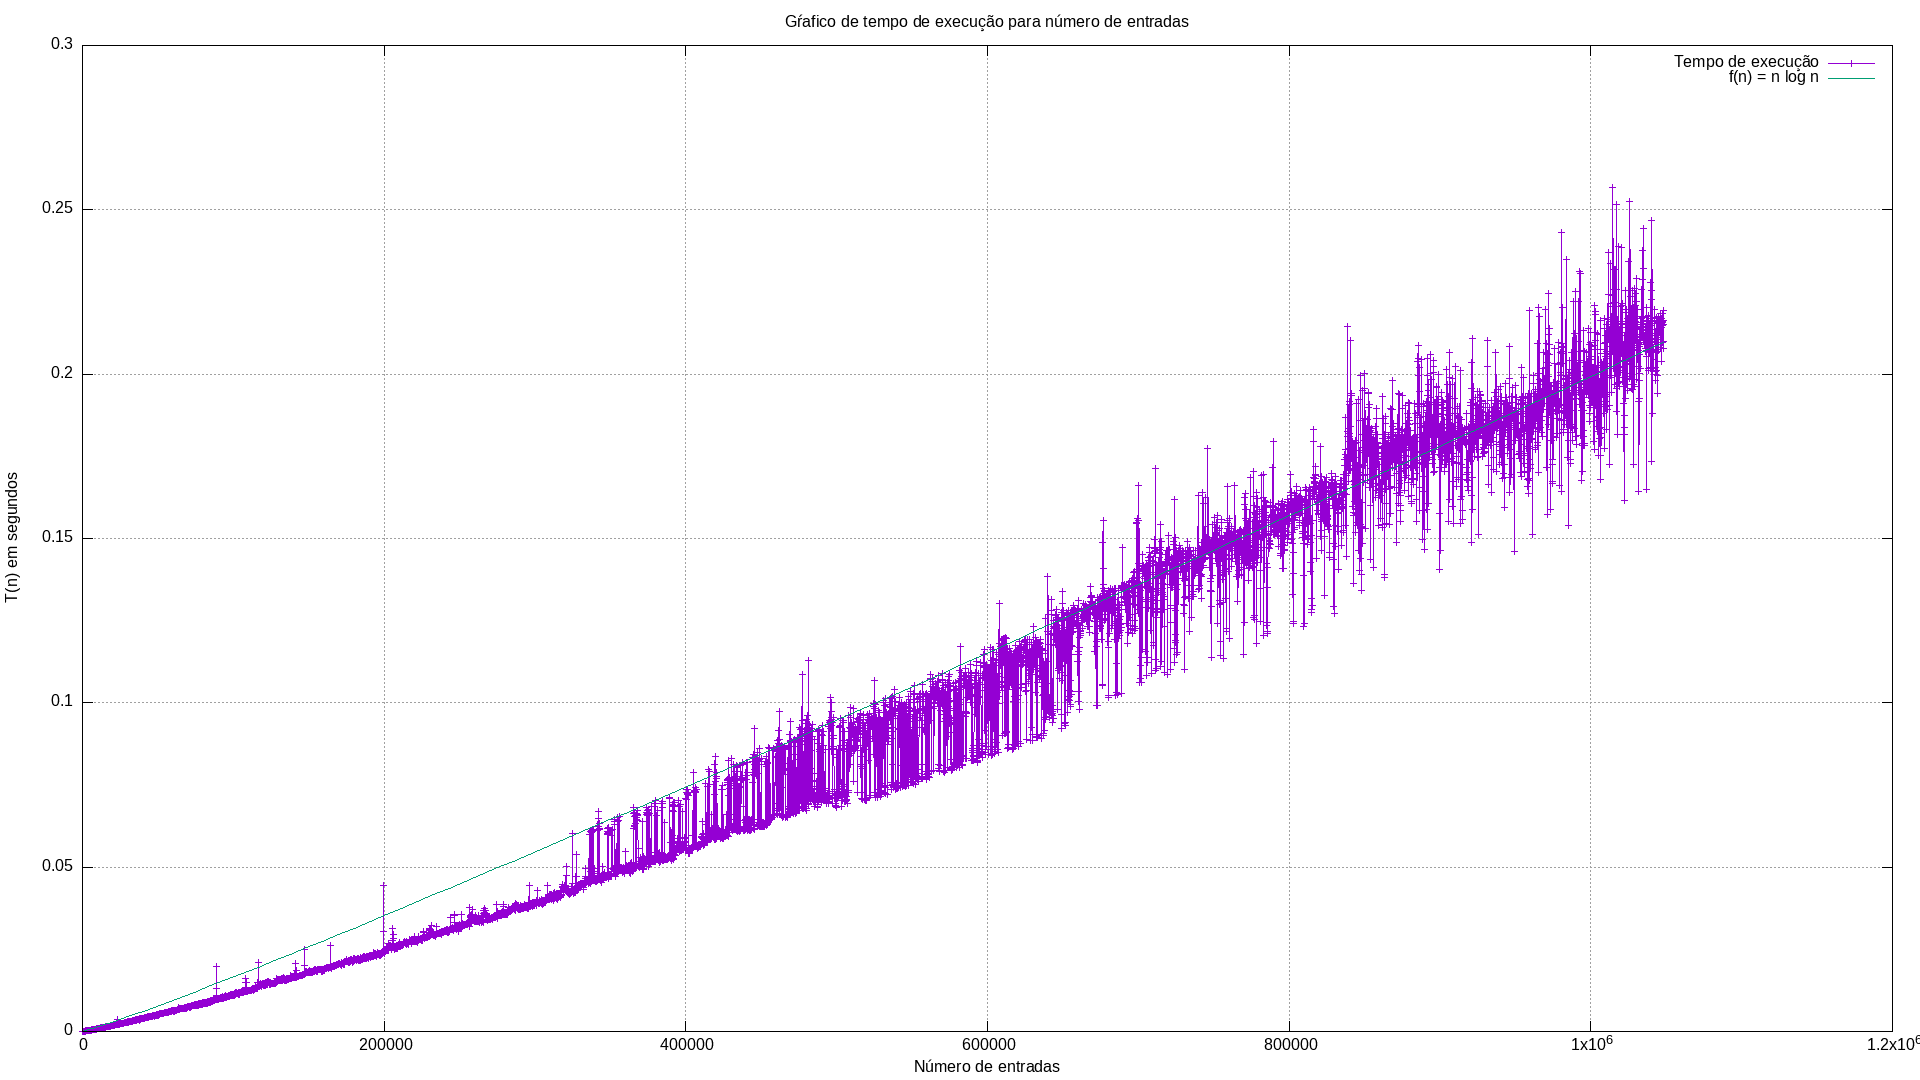
\includegraphics[width=\textwidth]{image/graphics/heapSort.png}
    \caption{Gráfico com tempo de execução do algoritmo de ordenação pela estrutura da \textit{Heap}}
    \label{cap:2:graph:heapSort}
\end{figure}

No gráfico \ref{cap:2:graph:heapSort}, é possível perceber que o tempo de execução do algoritmo se aproxima
da função $f(n)$ que é uma função $n \times \log n$ para $n$ com uma redução de escala para melhor percepção e comparação. Então,
utilizando como base o gráfico \ref{cap:2:graph:heapSort}, pode-se confirmar que a ordem de crescimento determinada é
precisa.

\subsection{Discussão sobre tempo de execução e uso de memória}

Sobre seu tempo de execução, o algoritmo de ordenação pela estrutura da \textit{Heap} é eficiente para
vetores com muitas entradas. Sobre seu uso de memória, é constante porque utiliza apenas algumas variáveis
auxiliares e transfigura o vetor origem de forma direta.

